
\chapter{Introduction} \label{chap:intro}

To understand on how the universe we live works is one of the most profound desire of human being. And this leads to all the creations all over from the mythology in history to the science in nowadays. Today, we believe that we understand this question, in particularly under the atomic scale, more clear than anytime in our history. All these knowledge about the physics laws in this universe can be summaries into a theory we called "Standard model". Although, this theory has archieved a great experimental success ever, there are questions and curiosities are still waiting to be answered. Besides several fundamental assumptions of the model are yet to be validated, knowing the behavior of a dihydrogen oxide atom well is far from enough to understand the wave in a ocean. Likewise, the phenomenon emerging from the collection of these fundamental particles can be non-trivial for us.



\section{The Standard Model}\label{sec:standard_model}
All the interactions we knew in the universe can be classifed into four types: the electromagnetism, weak interactoin, the strong interaction and gravity. The standard model provides a theory to describe three of them except the gravity. Based on the standard model, the bricks of the universe are individalbe fermionic particles which can be grouped into two classes: "quarks" and "leptons". Besides, several types of bosonic particles are playing the role of the interaction carrier to connect all elementary particles for building up the mechine of the current universe. All types of elementary particles in the standard model are illustrated in the Fig.~\ref{fig:standard_model_elementary_particles}. 

\begin{figure}[ht]
  \begin{center}
    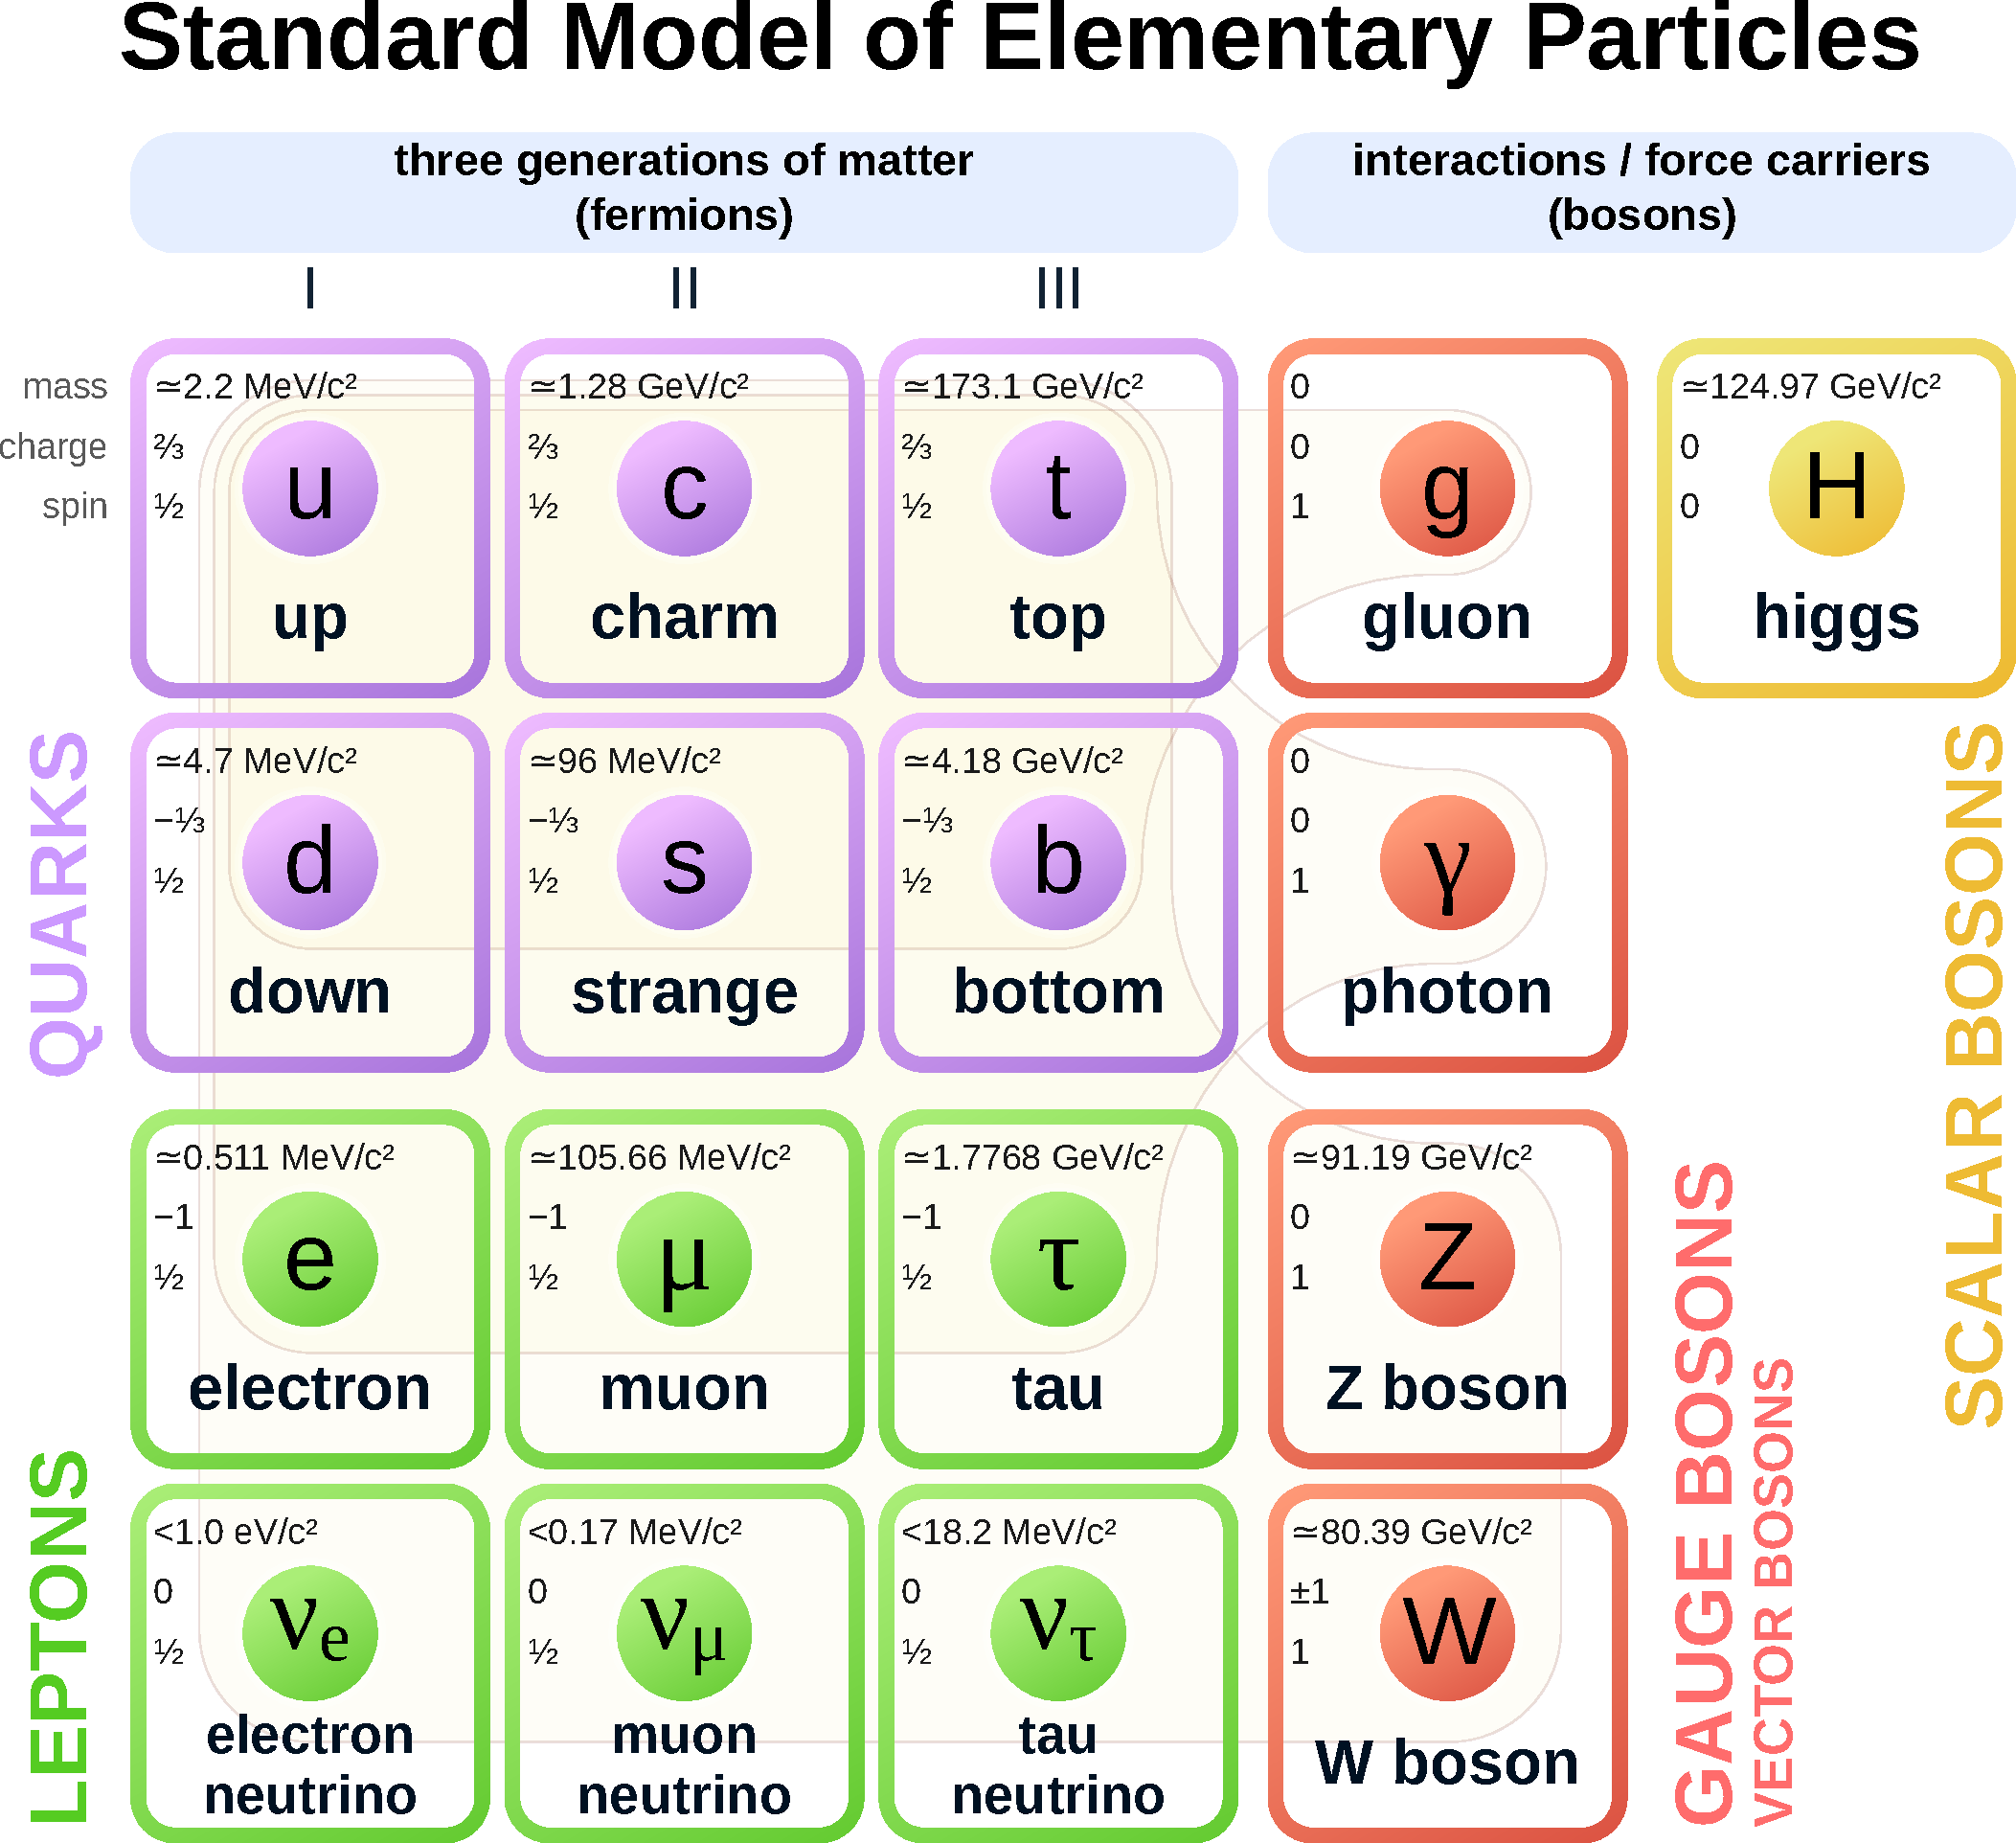
\includegraphics[width=0.8\textwidth]{figures/introduction/standard_model.pdf}
  \end{center}
  \caption{The pictorial representation of the elementary particles of the standard model.}
  \label{fig:standard_model_elementary_particles}
\end{figure}

The standard model suggested to group quarks and leptons into three generations, 2 particles for each quark or lepton generation in order to form the $SU(2)$ doublets. Each of particles process the isospin, weak hyper charge, and hence the electric charge. Besides of these quantum number, quarks carries color charges while the leptons don't. It means that the lepton will not participate the strong interaction. Unlike the quarks, each lepton is combined with a corresponding electric neutral neutrino to form a $SU(2)$ doublet. The neutrinos are considered to be left-handed massless particles while the modern experimental suggests that the chirality might be broken for them. All the leptons and quarks have anti-particles which have opposite electric charge to the original except the neutrino is anti-particle of itself. 

All the interactions are carried out by the gauge bosons: the photon $\gamma$ for the electromagnetism, the vector bosons $W^\pm$ and $Z$ for the weak interaction, and finally the gluon $g$ for the strong interaction. These gauge bosons corresponds to different gauge symmetries and only the electromagnetic $U(1)$ and colorful $SU(3)$ are preserved, so that the photon and gluon are massless. This electromagnetism $U(1)$ symmetry is broken from a $SU(2)\times U(1)$ symmetry by the Higgs mechanism which leads to the massive $Z$ and $W^\pm$. And this mechanism requires a non-vanished vacuum expectation of the Higgs field which is observed as the Higgs boson. 

While the electroweak theory gave a unified description on the electromagnetism and the weak interaction, the strong interaction is described by the Quantum Chromodynamics (QCD) in the standard model. Although both of the two theories build upon the non-Abelian gauge field theory, the different symmetry assumption leads to very distinguish consequence.

\subsection{The Quantum Chromodynamics}
The Lagrangian of the QCD can be illustrated as the formula below:
\begin{equation}
\mathcal{L}=i\bar\psi^i\slashed{D}^{j}_i\psi_j-m\bar\psi^i\psi_j-\frac{1}{4}G^a_{\mu\nu}G_a^{\mu\nu},
\end{equation}
where the $\psi^i$ are the quark fields and the $\slashed{D}=\gamma^\mu D_\mu$. 
\begin{equation}
\begin{aligned}
D_\mu&=\partial_\mu-i\frac{g_s}{2}G^a_\mu\lambda_a,\\
G^a_\mu&=\partial_\mu A_\nu^a-\partial_\nu A^a_\mu+gf^{abc}A^b_\mu A^c_\nu,
\end{aligned}
\end{equation}

where $\gamma^\mu$ are the Lorentz group, $g_s$ is the coupling constant, $A^a_\mu$ are the gluon fields and $f^{abc}$ are the structure constants of the $SU(3)$ group. Noticing the last term in the Lagrangian can leads to three or four self-coupling vertices for gluon fields. This feature not only increased the computation complexity for QCD processes, but also leads to unique QCD phenomenon.

The running coupling $\alpha_s(k^2)$ obtained from the one-loop renormalization is
\begin{equation}
\alpha_s(k^2) = \frac{4\pi}{\left(\frac{11N_C}{3}-\frac{2n_f}{3}\right)\ln\left(\frac{k^2}{\Lambda_{\text{QCD}}}\right)},
\end{equation}
leads to a feature that the coupling decreasing logarithmically as the $k^2$ raising, and this phenomenon is known as "asymptotic freedom". The $\lambda_{\text{QCD}}\sim200$ MeV which means that the coupling above this scale is expected to be weak (Fig.~\ref{fig:alphas}). This also implies that the coupling increasing with the decreasing of $k$ and makes the perturbation expansion with respect to the order of the coupling constant failed. However, the numerical calculation from lattice QCD suggested that the coupling between quarks will increasing linearly as a function of $r$, the distance between two quarks. This may explan the fact that there's no free quark observed in nature so far. And this experience is summarized to a postulation that partons are confined inside hadrons. 

\begin{figure}[ht]
  \begin{center}
    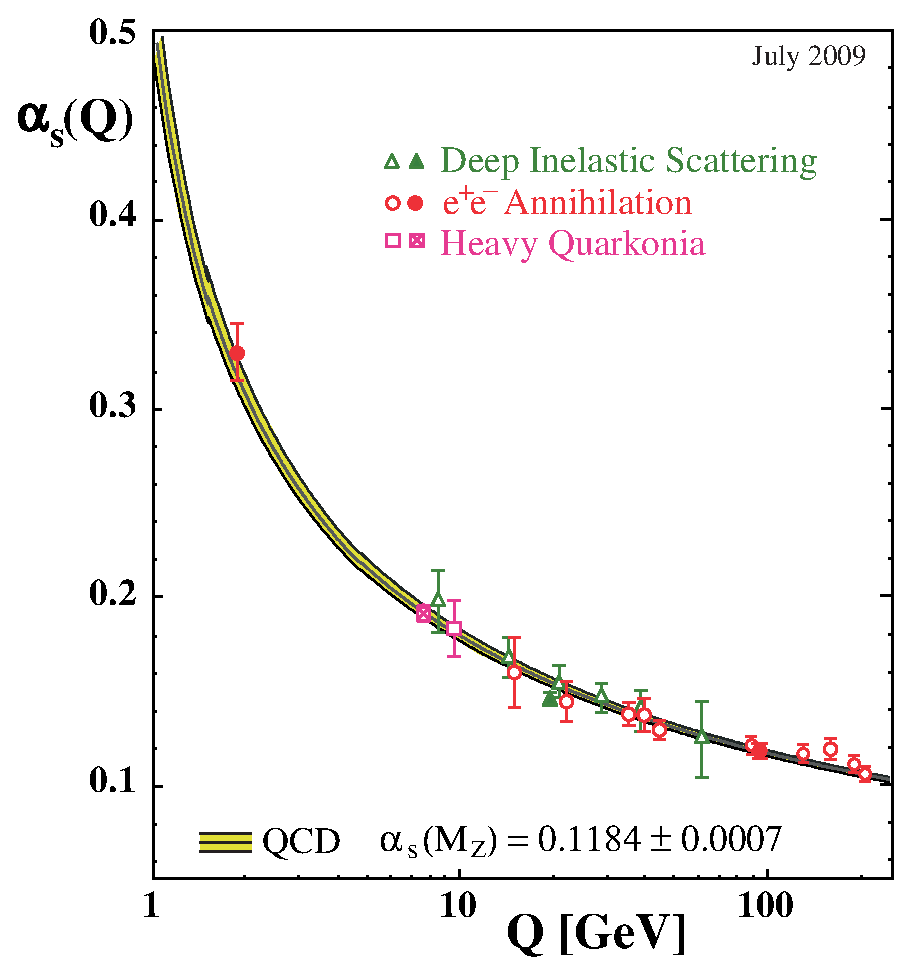
\includegraphics[width=0.5\textwidth]{figures/introduction/runing_alphas.eps}
  \end{center}
  \caption{The summary of the coupling constant measurements, as a function of the transverse momentum $Q$, from~\cite{Bethke:2012zza}.}
  \label{fig:alphas}
\end{figure}

\subsection{Hadron Collisions and Factorization}
The asymptotic free behavior leads to a simplification assumption that the collisions of two hadrons at high energy scale can be treated as the scattering of the partons from each of hadrons, like these partons are free relative to the rest constituents of the hadrons. This assumption works surprisingly well in deep inelastic scattering experiment. it suggests that the cross section of two hadrons $h_1,h_2$ to particles $X$ can be expressed as 
\begin{equation}
\begin{aligned}
\sigma(h_1h_2\to X)=&\sum_{n=0}^\infty\alpha_s^n(\mu_R^2)\int dx_1dx_2f_{i/h_1}(x_1,\mu^2_F)f_{j/h_2}(x_2,\mu^2_F)\\
&\times\sigma^{(n)}_{ij\to X}(x_1,x_2,\mu^2_R, \mu^2_F)+\mathcal{O},
\end{aligned}\label{eq:factorization}
\end{equation}
where $\alpha_s(\mu^2_R)$ is the coupling constant with the renormalization scale $\mu^2_R$, the $f_{i/h}(x,\mu^2_R)$ is the type $i$ parton distribution function (PDF) inside the hadron $h$, $x$ is the momentum fraction of the parton $i$ inside the hadron, and the $\mu^2_F$ is an arbitrary MS renormalization scale. However, this function can only be extracted from experiment or be calculated numerically based on DGLAP evolution.  $\sigma^{(n)}_{ij\to X}$ is the $n$-th order of the cross section of the process $ij\to X$.  The higher order represents the non-perturbation contributions.

The particles $X$ could be partons, however, due to the strong coupling of partons in long ranges, it is believed that the partons will be created and recombined together to form color singlet particles like hadrons. In that sense, the partons will continuous splitting into the partons through the QCD allowed vertices.


Suppose $f_{i/h}(x,\mu^2_F)$ stands for the amplitude that finding a parton $i$ from $h$ carrying the $z$ fraction of the energy of $h$, $\mu^2_F$ is an arbitrary normalization scale impling that this distribution includes all the contributions less than the scale $\mu^2_F$. However, if the energy increased by $\Delta Q$, then this distribution will needs to take the splitting contribution from the energy between $\mu^2_F$ to $\mu^2_F+\Delta Q$. This leads to the equation:
\begin{equation}
	\begin{aligned}
		f_{i/h}(x,\mu^2_F+\Delta Q)= f_{i/h}(x,\mu^2_F)+ \frac{\alpha(\mu^2_F)}{2\pi}\sum_jP_{i\leftarrow j}(z)f_{j/h}(x/z,\mu^2_F),
	\end{aligned}
\end{equation}
where $P_{i\leftarrow j}(z)$ represents the amplitude of a parton $i$ carried $z$ fraction of energy with respect to the parent parton $j$. And this leads to the Altarelli-Parisi Equation:
\begin{equation}\label{eq:DGLAP}
	\frac{\partial f_{i/h}(x,\mu^2_F)}{\partial \ln\mu^2_F} = \frac{\alpha(\mu^2_F)}{2\pi}\sum_j\int_x^1\frac{dz}{z}P_{i\leftarrow j}(z)f_{j/h}(\frac{x}{z}, \mu^2_F),
\end{equation}
where the splitting function can be obtained from pQCD order-by-order.

The energy of intial partons will be carried away by the branching partons until the energy fall below the branching threshold. The scattering between these partons will form into hadrons. The energy scale for this final stage is lower than the perturbative energy scale so that the higher order contriubtions are not negligible. The pQCD is no longer applicable in this stage so that we have to rely on some other models or effective theories.

%----------------------------------------------------------------------------------------
\subsection{QCD Branching , Hadronization and Jets}
Thinking of the evolution of a single initial parton, it will branching into multiple partons with less energies individually and this branching process will mixing a hadronization in the end period. The final observation we will get are a bunch of hadrons spatially distributed inside a small cone due to conservation of the momentum required these hadrons move into a roughly same direction. This collective observation is conceptually refereed as a "jet". Based on this conception, the definition of a jet can be detailed. Although the algorithm for clustering of these hadrons produced from the initial parton can be different which leads to the jet definition isn't unique. The factorization theorem tell us that these hadrons are closely related to the initial partons as we shown in Eq.~\ref{eq:factorization}. In this case, the function $f_{i/j}(z,\mu^2_F)$ can be understood as the fragmentation function and it still satisfies the DGLAP equation~\ref{eq:DGLAP} with a splitting kernel $P_{i\leftarrow j}(z)$. The expression of this kernel depends on the theory applicable on the energy scale $\mu^2_F$~\cite{Webber:1999ui}.

The splitting kernels for the partons in tree level are:
\begin{equation}
\begin{aligned}
P_{q\leftarrow q} (z) &= \frac{4}{3}\left[\frac{1+z^2}{(1-z)_+}+\frac{1}{3}\delta(1-z)\right],\\
P_{g\leftarrow q} (z) &= \frac{4}{3}\left[\frac{1+(1-z)^2}{z}\right],\\
P_{q\leftarrow g} (z) &= \frac{1}{2}\left[z^2+(1-z)^2\right],\\
P_{g\leftarrow g} (z) &= 6\left[\frac{1-z}{z}+\frac{z}{(1-z)_+}+z(1-z)+\bigg(\frac{11}{12}-\frac{n_f}{8}\bigg)\delta(1-z)\right],\\
\end{aligned}
\end{equation}
where the function $1/(1-z)_+$ is defined as:
\begin{equation}
  \int_0^1\frac{f(z)}{(1-z)_+}dz = \int_0^1\frac{f(z)-f(1)}{(1-z)}dz.
\end{equation}

Noticing that the singularity in the functions above are expected to be normalized when the higher order contributions are involved. The energetic parton will also lose energy by irradiating soft gluons. Suppose the $(d\sigma/d\Omega)_0$ stands for the cross section of the energetic parton production, with out considered the radiation. Then the summation over the soft gluon radiation will contribute a correction factor so that the measured cross section is
\begin{equation}
\begin{aligned}
  \left(\frac{d\sigma}{d\Omega}\right)_{\text{Phys.}} & = \left(\frac{d\sigma}{d\Omega}\right)_0\times\exp\left\{-\frac{\alpha}{\pi}f_{\text{IR}}(q^2)\log\bigg(\frac{-q^2}{\mu^2}\bigg)\right\}\\
  & \approx \left(\frac{d\sigma}{d\Omega}\right)_0\times\exp\left\{-\frac{\alpha}{\pi}\log\bigg(\frac{-q^2}{m^2}\bigg)\log\bigg(\frac{-q^2}{\mu^2}\bigg)\right\}
\end{aligned}
\end{equation}
where the $\mu$ is a infrared cut-off and the approximation hold for $q^2\gg m^2$. The coefficient $f_{\text{IR}}$ is:
\begin{equation}
  f_{\text{IR}}(q^2)=\int_0^1\left(\frac{m^2-q^2/2}{m^2-q^2 x(1-x)}dx\right)-1.
\end{equation}
The double logrithmic correction factor is known as Sudakov form factor. The probability of soft-gluon emission probability from a quark $Q$ is given by
\begin{equation}
  d\sigma_{Q\to Q g}= \frac{\alpha_s}{\pi}C_F\frac{(2\sin\theta/2)^2d(2\sin\theta/2)^2}{[(2\sin\theta/2)^2+\Theta^2]^2}\frac{d\omega}{\omega}(1+\mathcal{O}(\Theta)),
\end{equation}
where $\Theta = m_Q/E_Q\ll 1$ in relativistic case and $C_F$ is a color factor for the quark $Q$. For the case $\theta\ll 1$, the cross section is approximated to
\begin{equation}
   d\sigma_{Q\to Q g} \approx \frac{\theta^2d\theta^2}{(\theta^2+\Theta^2)^2}\frac{d\omega}{\omega},
\end{equation} 
which is a double logarithmic approximation. This implies that the cross section is suppressed in the region that $\theta<\Theta = M_Q/E_Q$. This effect can be significant if the mass of the quark is heavy such as the bottom or top quark. This suppression is known as dead cone effect, and it leads to the depopulation and leading parton effect to heavy flavor jets~\cite{Dokshitzer:1991fd}.

%----------------------------------------------------------------------------------------
\section{QCD Phase Transition and Quark-Gluon-Plasma}

We knew that a hadron is formed by the partons bundling by the strong interaction propagated through gluons. The effective potential between a pair of $q\bar q$ is approximated by
\begin{equation}
V(r) = -\frac{A\cdot\ln r}{r}+K\cdot r,
\end{equation}
where $r$ is the distance between the two quarks and $A,K$ are constants~\cite{Hands:2001ve}. The asymptotic freedom happens when $r\to 0$ and the color confinement ensured by the linear term in the potential. Based on this idea, the Bag model is proposed to describe the hadron energy phenomenologically: a hadron energy density should be almost constant within a certain region with radius $R$, the hadron size, while the energy decrease outside this region. Based on this idea, the energy density of a hadron is approximated by

\begin{equation}
E \propto R^3\Lambda_B^4 + \frac{C}{r},
\end{equation}
where the second term comes from the potential. The mass of this hadron is given by minimum point of $R$ in this equation: $M\sim 3\Lambda^4_BR^3$. For a typical value $R\sim1$~fm and $M\sim 1000$~MeV, the bag energy density is about $\Lambda^B\sim200$~MeV.

The binding from strong coupling will be broken if the partonic kinematic energy inside of the hadron is large enough. Partons will be created along with the gluon string breaking and hence the degree of the partonic freedom will increase. This parton creation process will reduce the kinematic energy to form new bound states. But the baryon number is conservative in QCD interaction so that the QCD matter system can be described by a grand canonical ensemble $E-TS-\mu_BB$ where $S, T, B, \mu_B$ are the entropy, temperature, net baryon number, and the baryon chemical potential, respectively. The ensemble of these hadrons formed a gas-like phase of hadrons and the Stefan-Boltzmann's law is applicable. However, if the energy density is keeping increasing, it will leads to the partonic density increases so that the mean free pass length is getting shorter. The screening effect from the saturated partons will weaken the confinement of the partons so that they might eventually be free. The lattice QCD calculation shows that the Stefan-Boltzmann's law is broken around the $T=150$~MeV, Fig.~\ref{fig:lattice_phase_transition}. The raising entropy, which means extra number of the micro-states occurs, is contributed by the new degree of freedom from the de-confined partons. This non-trivial changes implies the system reaches a new phase known as quark-gluon plasma (QGP), analogous to the plasma discovered for electron and ions. The 4th power of temperature law is restored after $T>500$~MeV due to the partons are completely free and no extra degree of freedom can be added into the system. After the phase transition, the effective potential $V_{QGP}(r)$ for $q\bar q$ is

\begin{equation}
  V_{QGP}(r)=-\frac{C}{r}\exp\left(-\frac{r}{\lambda_D}\right),
\end{equation}
where the $\lambda_D(T)\propto 1/T$ is the Debye screening length due to the color charges are surrounded by soft color particles, like the naked color charge disappeared. The string term disappears due to the confinement string is broken. The Debye screening length for $T>T_c$, where $T_c$ stands for the critical temperature for QCD phase transition to happen, is about $\lambda_D\sim O(0.1)$~fm~\cite{Kajantie:1997pd}.

\begin{figure}[ht]
  \begin{center}
    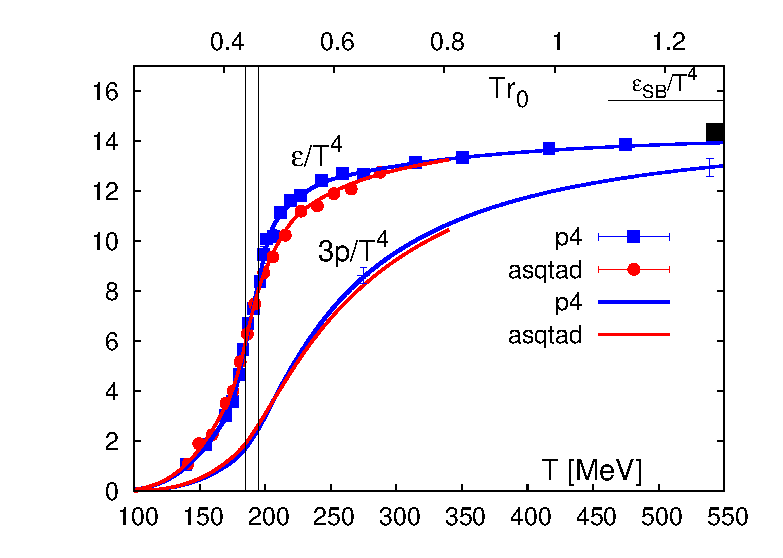
\includegraphics[width=0.8\textwidth]{figures/introduction/energy_3p_MeV_p4_asqtad.eps}
  \end{center}
  \caption{The energy density and the 3 times the pressure divided by the fourth power of the tempreture of QCD matters. A cross over transition happened around $T=170$ MeV and slowly converge to the Stenfan-Boltzman's law after $T>500$ MeV~\cite{Bazavov:2009zn}.}
  \label{fig:lattice_phase_transition}
\end{figure}

\subsection{Relativistic heavy-ion collisions}
The accelerator technique can be used to compress hundreds of atoms into a very small space to reach the critical temperature of QCD phase transition. The fixed target experiments performed at the Alternating Gradient Synchrotron (AGS) in Brookhaven and the Super Proton Synchrotron (SPS) at CERN are the first two experiments attempting to artificially create the QGP between 1986 and around 2000. The center-of-mass energy per nucleon pair $\sqrt{s_{\text{NN}}}$ is 10~GeV and 20~GeV at the AGS and SPS, respectively. These measurements shows the evidence of the fraction of strangeness hadron enhancement in the final production compared to smaller collision systems. Furthermore, the measurement from SPS observed the suppression of $J/ \psi$ meson yields~\cite{Heinz:2000bk} which is confirmed by the later measurements at Relativistic Heavy Ion Collider (RHIC). Furthermore, they also observed the yield suppression generally exists for all particles with high transverse momentum. These phenomenon is collectively summarized as "jet quenching"~\cite{Adams_2006,Bjorken:1982tu,Adare:2007vu}. These evidence confirmed that QGP can be and was created in the heavy-ion collisions. Anther evidence comes from the measurement revealed a non-uniform soft particle momentum distribution as a function of the azimuthal angle $\phi$ which is known as elliptic flow~\cite{Ackermann:2000tr}. This is a phenomenon often exists in a long range correlation dominated system described by hydrodynamics. 

It is found that the Glauber model describes the hard processes in relativistic heavy-ion collisions well. Based on this model, a heavy-ion nuclei can be approximated by a bunch of nucleons superposition with respect to a nucleon wave function $\phi(r)$. The collision of two nuclei are considered as the collision of those two bunches of nucleons and the nucleon-nucleon interaction within the nuclei itself is ignored. Due to the Lorentz contraction, the collision of two ions is like the collision of the two discs with the centers offset by a distance from each other. We use a vector $\boldsymbol{b}$ (impact parameter) originated from the center of ion $A$ pointing to the center of ion $B$ to quantify this collision geometry. The nucleon density of a ion $A$ is rewritten into a thickness function $T_A(\boldsymbol{s})$ where the $s$ is the distance vector from the center to any point on the disc. Only those nucleons in the overlap region will participant the collision and the number of them is noted as $N_{\text{part}}$. The probability $P(n,\boldsymbol{b})$ to have $n$ hard collisions between ions $A,B$ is given by the binomial distribution
\begin{equation}
  P(n,\boldsymbol{b})=\binom{AB}{n}
  \left[\hat T_{AB}(\boldsymbol{b})\sigma_{\text{NN}}^{\text{intel}}\right]^n\left[1-\hat T_{AB}(\boldsymbol{b})\sigma_{\text{NN}}^{\text{intel}}\right]^{AB-n},
\end{equation}
where the $\sigma_{\text{NN}}^{\text{intel}}$ is the nucleon-nucleon cross section. The $A,B$ are the nucleon number of each ions and the $T_{AB}(\boldsymbol{b})$ is the overlap thickness function defined as
\begin{equation}
  \hat T_{AB}(\boldsymbol{b})=\int d^2s \hat T_{A}(\boldsymbol{s})\hat T_B(\boldsymbol{s}-\boldsymbol{b}).
\end{equation} 

The total nuclei-nuclei cross section $\sigma_{NN}$ comes from summation over the binomial distribution
\begin{equation}
  \sigma_{\text{NN}} = \int 2\pi b db \left\lbrace 1-\left[1-\hat T_{AB}(b)\sigma^{\text{NN}}]_{\text{intel}}\right]^{AB}\right\rbrace.
\end{equation}
Further more, the number of the hard nucleon-nucleon collisions is given by
\begin{equation}
  N_{\text{coll}}(b) = \sum_{n=0}^{AB}nP(n,\boldsymbol{b})=AB \hat T_{AB}(\boldsymbol{b})\sigma_{\text{NN}}^{\text{intel}},
\end{equation}\label{eq:ncoll}
where $AB$ can be put into the overlapping function that $T_AB=AB\hat T_AB$.


The nucleon-nucleon cross section $\sigma_{\text{NN}}^{\text{intel}}$ is modeled the same way as~\ref{eq:factorization} with a nucleon PDF(nPDF). The difference between the PDF and nPDF can result variety phenomenons like the color nuclear matter effects, for instance. 

The different between the $\sigma_{\text{NN}}^{\text{intel}}$ and the free hadron cross section $\sigma$ can be quantified by the ratio of the differential particle yield $R_{AB}$:

\begin{equation}
  R_{AB}(x)=\frac{1}{\langle N_{\text{coll}}\rangle}\frac{dN^{AB}/dx}{dN^{pp}/dx} = \frac{1}{\langle T_{AB}\rangle}\frac{dN^{AB}/dx}{ d\sigma/dx},
\end{equation}
where $A,B$ stands for the type of the two colliding particles and $x$ can be any observables like $\pt, \eta, \Omega$, etc. It is worth to notice that the measurement of $T_{AB}$ usually has less uncertainty than $N_{\text{coll}}$. A variety measurement on the nuclear modification factor of photon or $W,Z$ bosons shows no significant difference between the $\sigma_{\text{NN}}^{\text{intel}}$ and $\sigma$ for the electro-weak processes~\cite{Sirunyan:2020ycu,Aad:2019lan,Aad:2019sfe}. Because of the weak particles won't be affected significantly by the QGP which major involves strong interactions, these measurements proves that the Glauber model successfully described the collision geometry and the size of the hard scattering. Besides the effect from QGP, the nPDF of a nucleon is different from the same type of hadron. This difference can be extracted from the nuclear modification factor of other collision system such as $R_{pA}$ or $R_{eA}$ where the QGP effect is relatively small or negligible~\cite{Kusina:2015vfa}. The relative modification of the hadron in nuclei can result the color nuclear matter effects~\cite{Arneodo:1992wf}.

%----------------------------------------------------------------------------------------
\subsection{Jet Quenching and Hard Probes}
The typical size of the QGP is a few fm (estimated 6-11~fm at LHC) and the formation time of QGP is less than 1~fm/$c$~\cite{Liu:2012ax} which implies that part of jets will path through this hot medium. As we mentioned previously, the $R_{AA}(\pt)=1$ for weak particles like photon or $Z$ bosons. However, as an example shown in the Fig~\ref{fig:cms_charged_particle_Raa}, the $R_{AA}(\pt)<1$ for high $\pt$ particles and jets means the energy observed from these particles is relatively softer than those in pp collisions. Additionally, the imbalance study on photon-tagged jets in Fig.~\ref{fig:cms_gamma_jet} shows that the jets lost energy in heavy-ion collisions.

\begin{figure}[ht]
  \begin{center}
    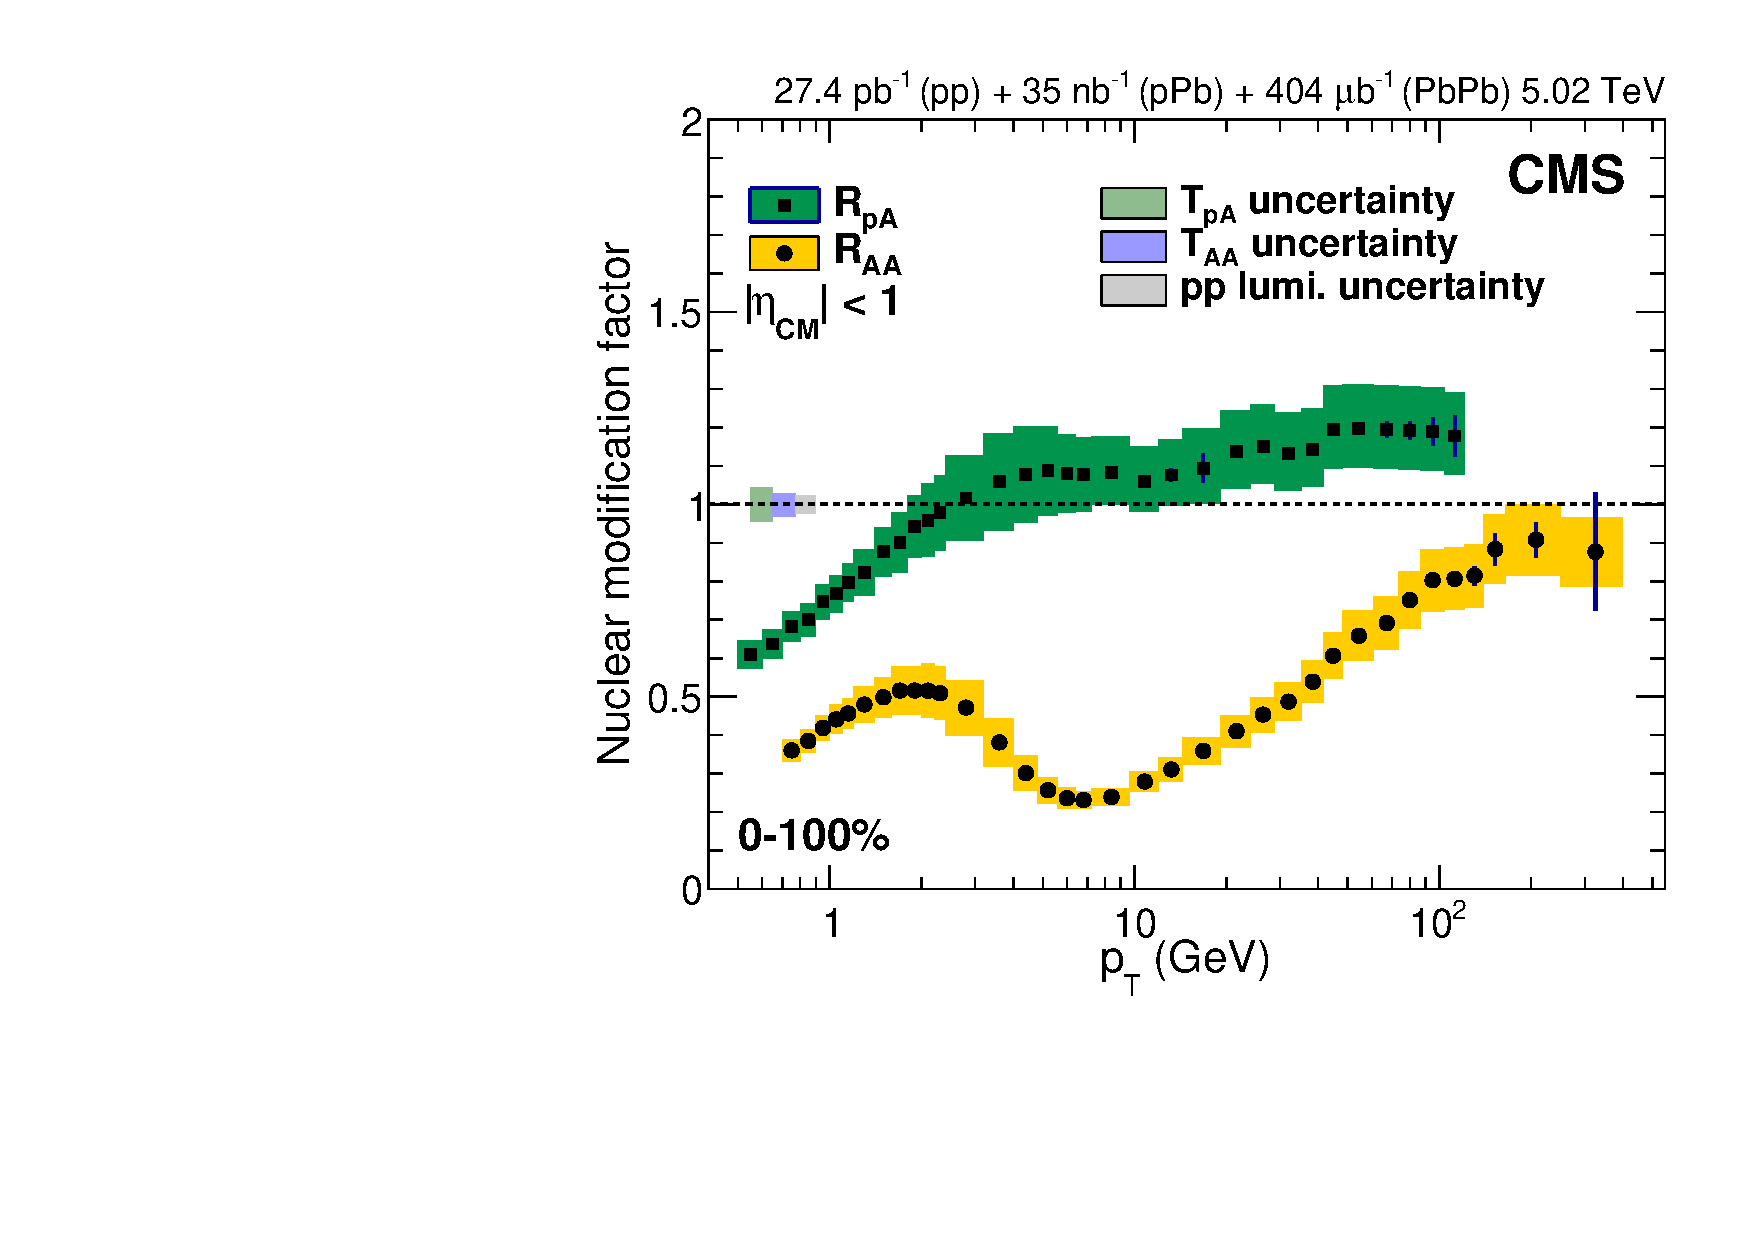
\includegraphics[width=0.6\textwidth]{figures/introduction/Charged_Particle_RAA.pdf}
  \end{center}
  \caption{The nuclear modification factor for inclusive charged particle produced in PbPb and pPb collisions measured by the CMS collaboration. The $R_AA(\pt)<1$ for high $\pt$ particles in PbPb collisions~\cite{Khachatryan:2016odn}.}
  \label{fig:cms_charged_particle_Raa}
\end{figure}

\begin{figure}[ht]
  \begin{center}
    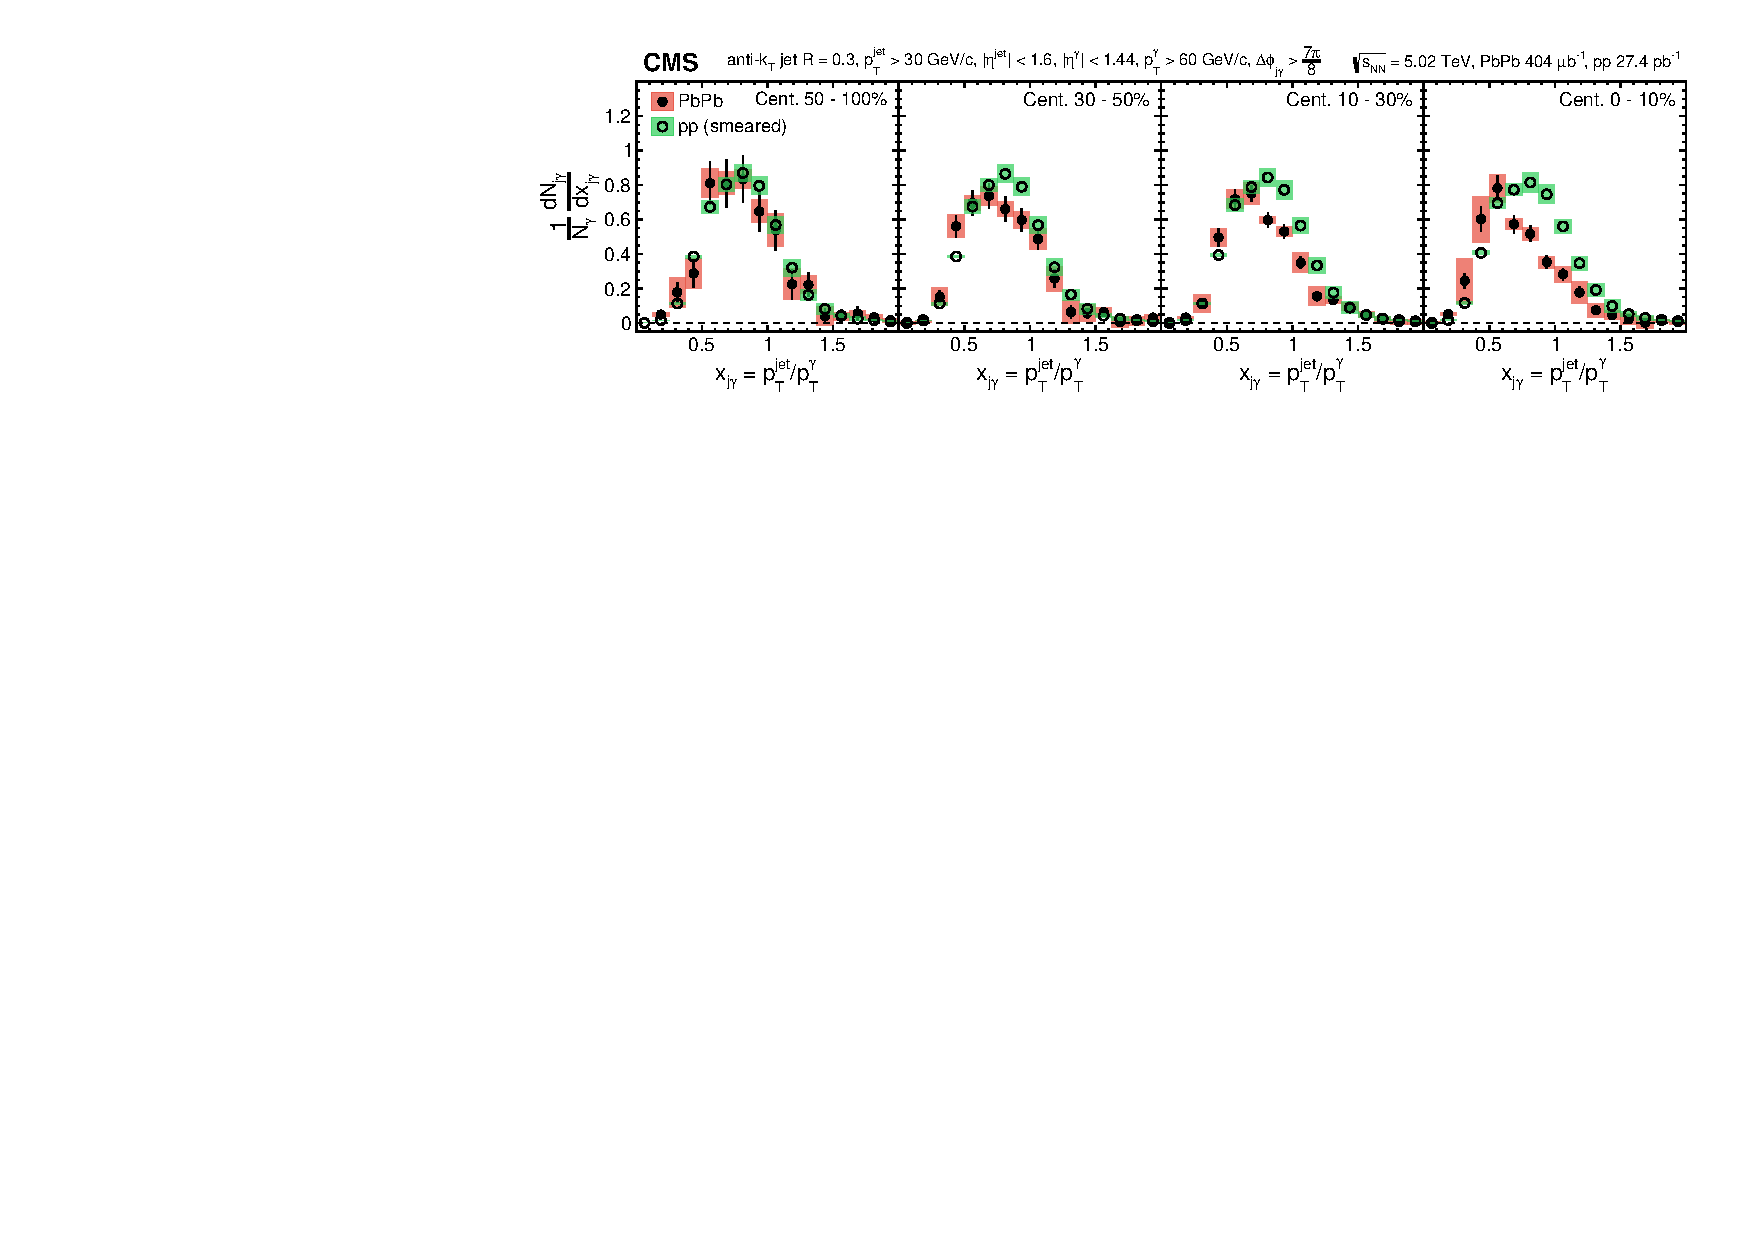
\includegraphics[width=\textwidth]{figures/introduction/CMS-HIN-16-002_Figure_006.pdf}
  \end{center}
  \caption{The transverse momentum ratio $X_{j\gamma}$ of $\pt^{\text{jet}}$ to $\pt^{\gamma}$ for differential centrality bins and compared with that in pp collisions~\cite{Sirunyan:2017qhf}. The $X_{j\gamma}$ is almost the same in pp and peripheral PbPb collisions, but the $X_{j\gamma}$ shifted significantly to the soft sector in PbPb central collisions.}
  \label{fig:cms_gamma_jet}
\end{figure}

Providing the fact that the jet production and evolution is well described by pQCD, these evidence not only prove that the QGP is created in heavy-ion collisions, but also allow us to use jets as probes to study the properties of this hot medium. Theoretically, the leading order term of the hard scattering in heavy-ion collisions can be obtained from the factorization Eq.~\ref{eq:factorization} with a modification term $\mathcal{P}(ab\to cd|T,u^\mu)$:
\begin{equation}
\begin{aligned}
  \sigma(h_1h_2\to X)&=\alpha_s(\mu_R^2)\int dx_1dx_2f_{i/h_1}(x_1,\mu^2_F)f_{j/h_2}(x_2,\mu^2_F)\\
&\times\sigma^{(1)}_{ij\to ab}(x_1,x_2,\mu^2_R, \mu^2_F)\\
&\times\mathcal{P}(ab\to cd|T,u^\mu)D_{X\leftarrow cd}(z_c,z_d,\mu^2_F),
\end{aligned}
\end{equation}
where the $D_{X\leftarrow cd}$ is the fragmentation function describing the hadrons $X$ fragmented from energetic partons $c,d$, and $T,u^\mu$ stands for the temperature and the flow viscosity of the medium. The new term $\mathcal{P}(ab\to cd|T,u^\mu)$ stands for the probability amplitude of the partons $a,b$ transfer into $c,d$ due to the interaction with the medium (through a multi-scattering process illustrated in Fig.~\ref{fig:multi_scattering_in_medium}. Rather than that, the fragmentation term $D_{X\leftarrow cd}(z_c,z_d,\mu^2_F)$ maybe different from the case in vacuum. This fragmentation function still satisfies the DGLAP equation with a kernel of the parton interaction in medium which build a bridge to understand the QGP properties by studying the jet modification in heavy-ion collisions. z

\begin{figure}[ht]
  \begin{center}
    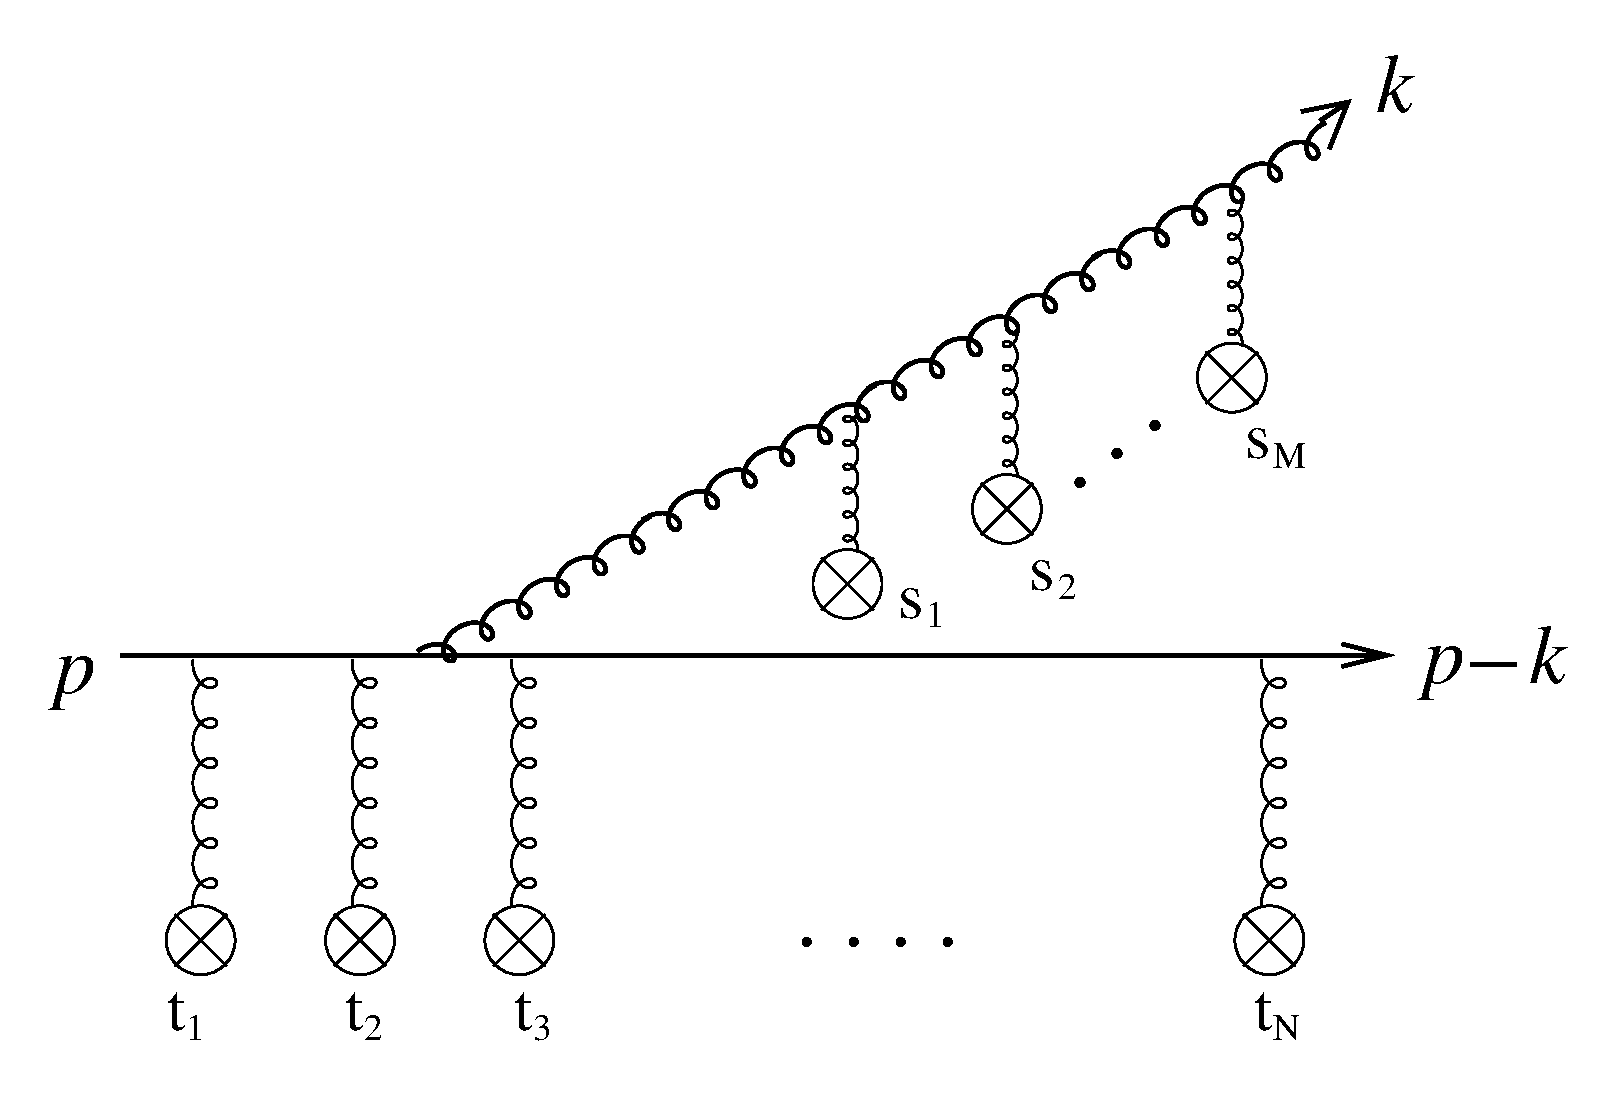
\includegraphics[width=0.6\textwidth]{figures/introduction/multi_scattering_in_medium.eps}
  \end{center}
  \caption{The schematic illustration of a energetic parton scattering process when medium presents, taking from~\cite{Jeon:2009yv}. The source term refers the interaction from the QGP.}
  \label{fig:multi_scattering_in_medium}
\end{figure}

Jet structure measurements can be used to constraint the branching kernel so that providing more detailed information to understand the QGP properties. The jet shape which is the jet constituent $\pt$ distribution around the jet as a function of the distance of the constituent from the jet axis $r=\sqrt{(\Delta\eta)^2+(\Delta\phi)^2}$, where $\Delta\eta= \eta_{\text{particle}}-\eta_{\text{jet}}$ and $\Delta\phi= \phi_{\text{particle}}-\phi{\text{jet}}$ is measured for inclusive jets~\cite{Sirunyan:2018jqr}. The comparison between the jet shapes in PbPb and pp shows that the energy has been shifted from higher $\pt$ bin to lower bins, and the energy distributed in larger $\Delta r$ region is higher than that in pp collisions. These modification shows clear centrality dependence which may related to the path length of the initiate parton of the jet (Fig.~\ref{fig:inclusive_jet_shapes}.

\begin{figure}[ht]
  \begin{center}
    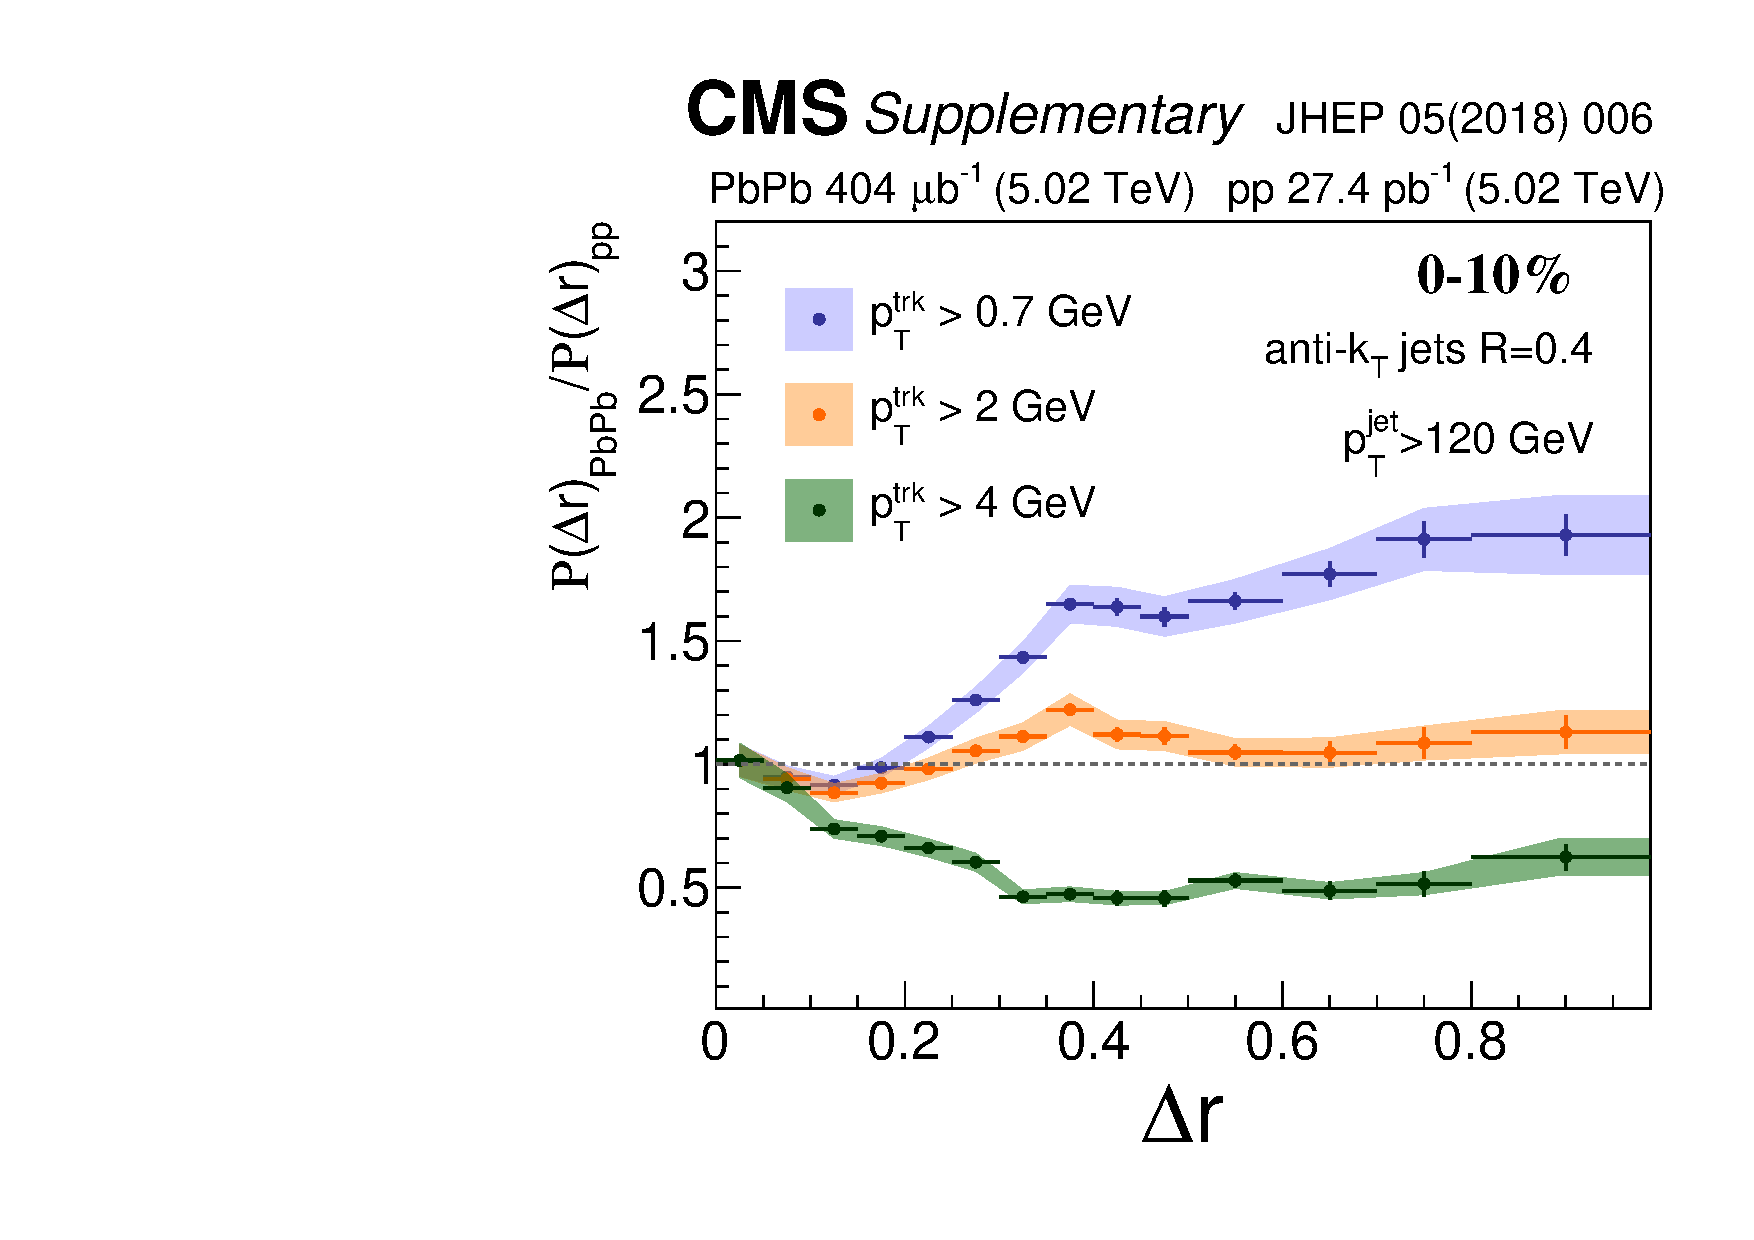
\includegraphics[width=0.5\textwidth]{figures/introduction/CMS-HIN-16-020.pdf}
  \end{center}
  \caption{The ratio of the radial jet momentum distribution $P(\Delta r)$ of jets between PbPb and pp collisions for the indicated intervals of $\pttrk$ shown for the 0-10\% (most central) bin. The shaded bands show the total systematic uncertainties~\cite{Sirunyan:2018jqr}.}
  \label{fig:inclusive_jet_shapes}
\end{figure}

The branching of the initial quarks will leads to one energetic jet split into two or more sub-jets carry portion of the energy from the original one. This process is a consequence phenomenon of the DGALP equation. This process should be infrared (IR) safe for the summation of all order of contribution but it is ill-defined to any certain order of $\alpha_s$. With a jet grooming method, the IR unsafe part of the splitting function can be removed so that the rest part can be approximated by pQCD calculation. The observable splitting function is a distribution of function $z_g$
\begin{equation}
  z_g= \frac{\text{min}(\pt_1,\pt_2)}{\pt_1+\pt_2}.
\end{equation}
The measurement of $z_g$ removed the soft splitting by the grooming condition $z_g>0.1$ shows that the $z_g$ distribution of the peripheral PbPb collisions is similar to the pp collisions which is well simulated by the PYTHIA and Herwig++ generator. However, the $z_g$ in central PbPb collisions is modified to a softer splitting side (smaller $z_g$) comparing to pp collisions (Fig.~\ref{fig:splitting_function}).

\begin{figure}[ht]
  \begin{center}
    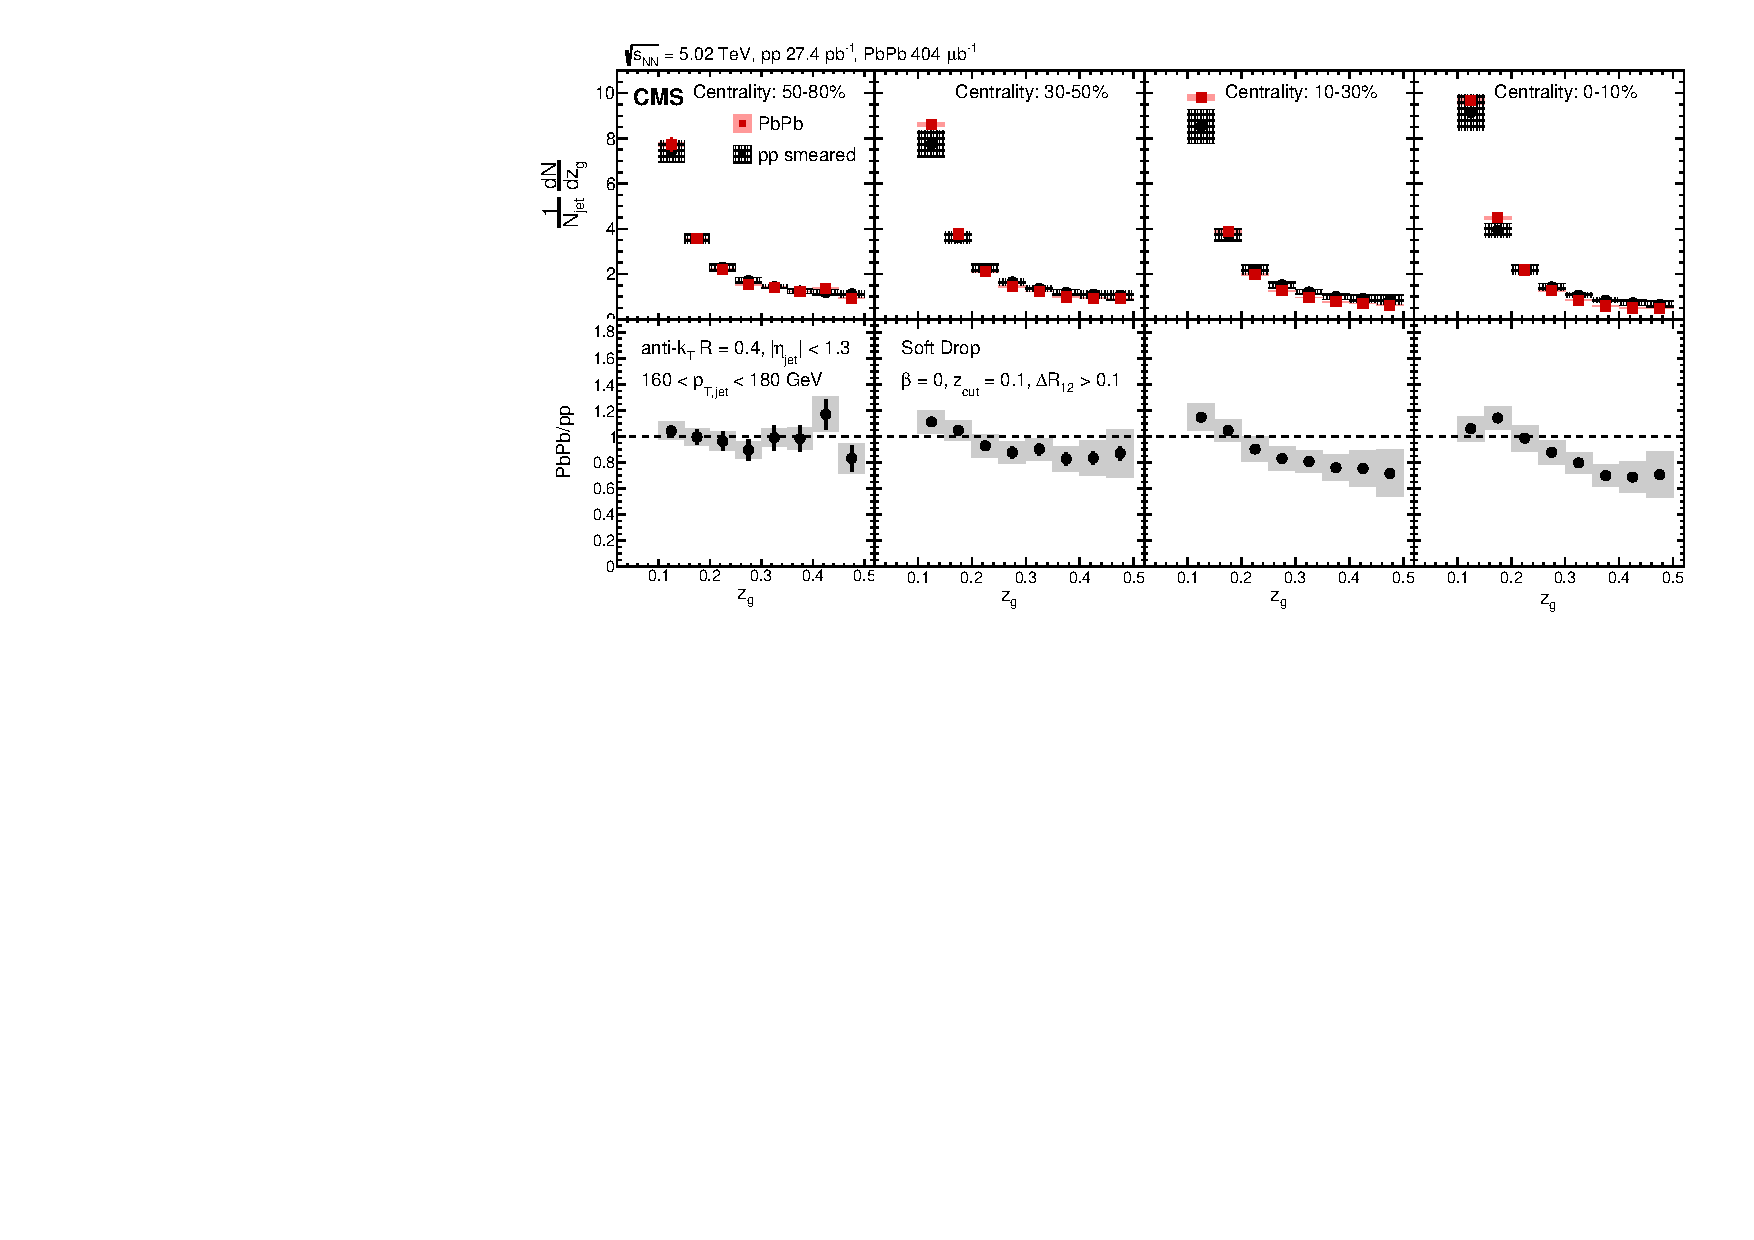
\includegraphics[width=1\textwidth]{figures/introduction/CMS-HIN-16-006_Figure_003.pdf}
  \end{center}
  \caption{The splitting function in PbPb collisions shown in differential centrality bins and overlay with the smeared splitting function in pp collisions. Taken from~\cite{Sirunyan:2017bsd,}.}
  \label{fig:splitting_function}
\end{figure}

The heavy flavor jets which are those jets initiated by a heavy flavor parton like, c, b or t quarks plays a unique role in the jet tomography probing the QGP properties. Because of the large mass of heavy flavor quarks, they are severely suppressed from the medium thermal production and will have to be created mainly from the very early hard scattering. The evolution of the heavy flavor jets will carry a full information of space-time profile and the transportation properties of the QCD medium. Besides of this, the energy loss of the heavy flavor partons are expected to be less compared to the lighter partons due to the mass hierarchy. However, recent measurement shows a contradictory result: the jet imbalance study on b jet pairs show similar $X_J$ distribution as inclusive jet pairs~\cite{Sirunyan:2018jju}. The suppression level of the prompt D meson nuclear modification factor $R_{AA}$ is almost comparable with the inclusive charged particles~\cite{Sirunyan:2017xss}. These collective counter intuitive observation is collectively known as "heavy flavor puzzle". On the other hand, some heavy flavor jets can produced pairwise from a gluon splitting process. Although the splitting kernel is not IR safe but with grooming method, it can be a excellent observable to test the pQCD. Since some studies suggests the jet substructure might be very non-trivial in heavy ion collisions~\cite{Li:2017wwc}, It also can be used to test any potential changes of the pQCD in a finite temperature environment. More subtle heavy flavor jet structure measurements are needed to solve these questions. 